% Created 2022-01-27 Thu 10:44
% Intended LaTeX compiler: pdflatex
\documentclass[11pt]{article}
\usepackage[utf8]{inputenc}
\usepackage[T1]{fontenc}
\usepackage{graphicx}
\usepackage{longtable}
\usepackage{wrapfig}
\usepackage{rotating}
\usepackage[normalem]{ulem}
\usepackage{amsmath}
\usepackage{amssymb}
\usepackage{capt-of}
\usepackage{hyperref}
\usepackage{color}
\usepackage{listings}
\usepackage{color}
\usepackage{listings}
\author{Maikol Solís}
\date{\textit{<2022-01-27 Thu>}}
\title{Emacs workshop 2022: Day 4}
\hypersetup{
 pdfauthor={Maikol Solís},
 pdftitle={Emacs workshop 2022: Day 4},
 pdfkeywords={},
 pdfsubject={},
 pdfcreator={Emacs 27.2 (Org mode 9.6)}, 
 pdflang={English}}
\usepackage{biblatex}

\begin{document}



\section{Handling knowledge with Emacs}
\label{sec:org5a9ea94}

\subsection{The Zettelkasten method}
\label{sec:org4e96c27}

Niklas Luhmman wrote 70 books and nearly 400 scholarly articles published on a variety of subjects, including law, economy, politics, art, religion, ecology, mass media, and love.

\begin{center}
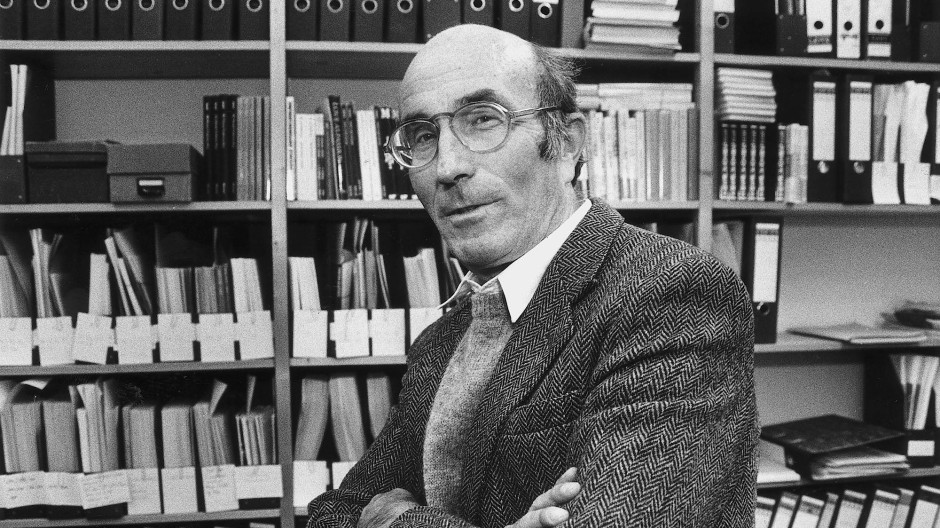
\includegraphics[width=15em]{./nl.png}
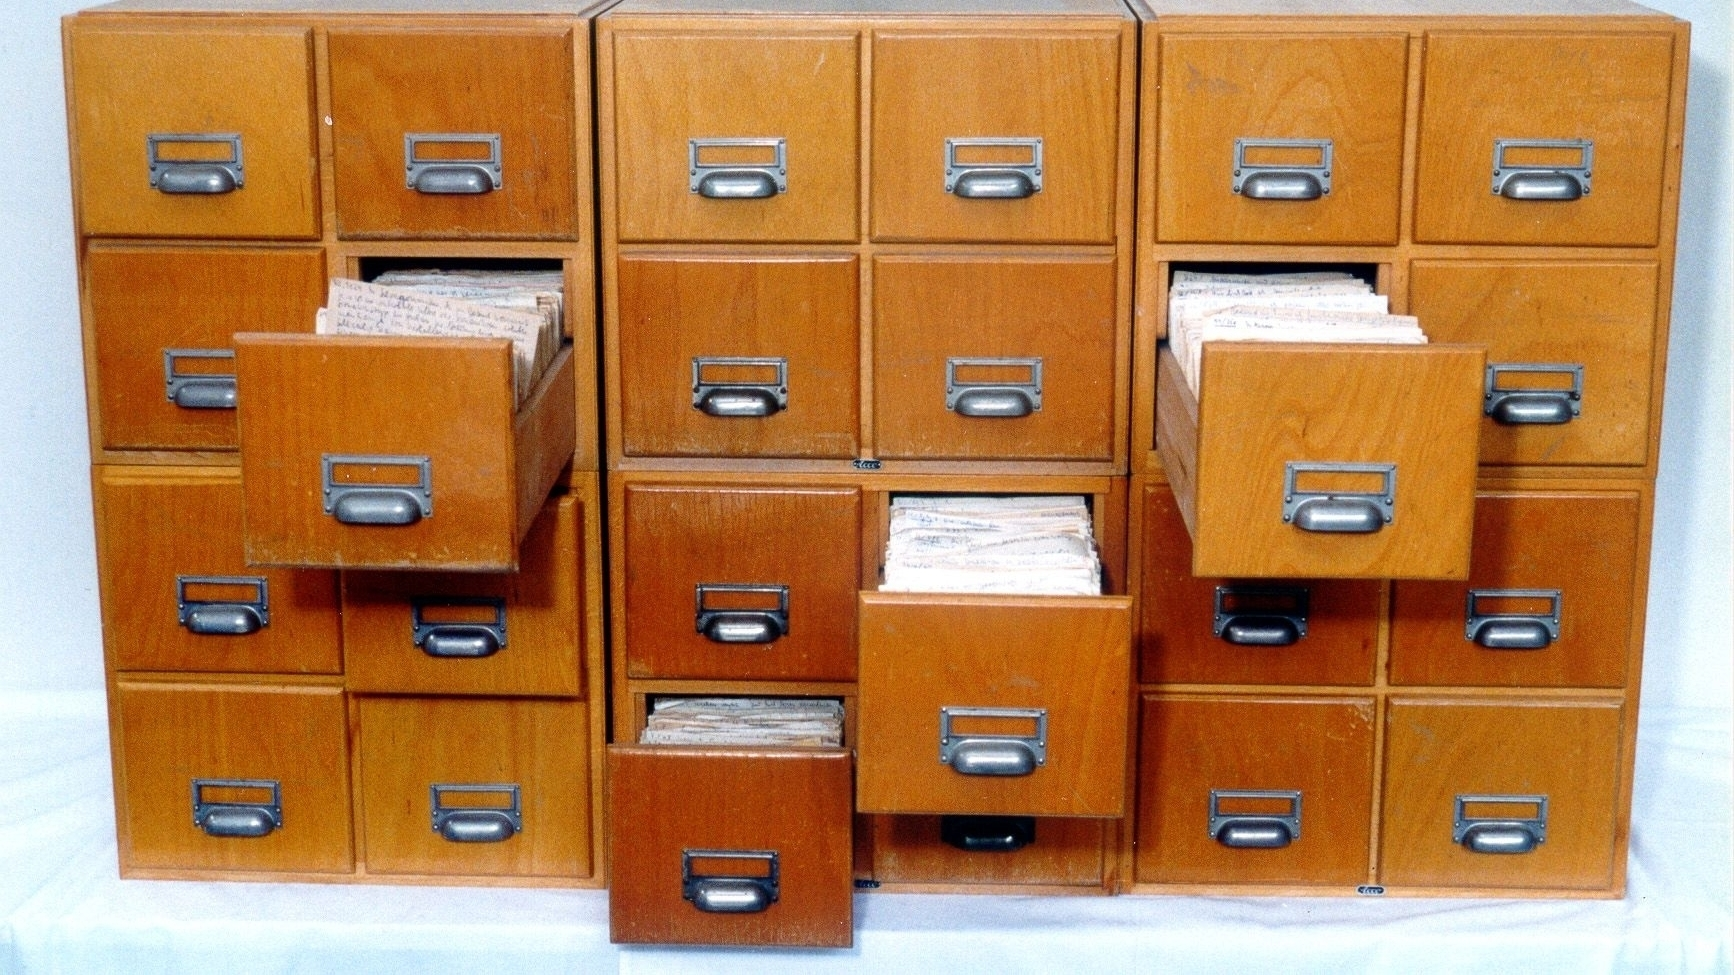
\includegraphics[width=15em]{./zk.png}
\end{center}

\subsection{Why?}
\label{sec:orgc70237b}

\begin{itemize}
\item Improved understanding of the concepts
\item Better retention and recall
\item You'll find links between concepts that were not apparent before
\item Intentionality - you'll be more focused when learning because you have to think and make notes
\item You have one place to store all your notes - not spread across multiple platforms
\end{itemize}


\subsection{The process}
\label{sec:org2aaf6c8}

The Zettelkasten process has three types of notes\ldots{}

\subsubsection{Fleeting Notes}
\label{sec:orgbf37a7b}

Incomplete ideas, memory reminders

\subsubsection{Literature Notes}
\label{sec:orga592402}

After reading a papers or books you need to include  the references and expand the fleeting notes into more structured note.

These are notes about other's ideas.


\subsubsection{Permanent Notes}
\label{sec:orga12d5ca}

Once you have finished with your literature notes, you need to extract every idea/concept into separate notes.


\begin{itemize}
\item Write only one idea per note but be as complete as possible. This forces you to think about the content and distill it down to its core ideas.
\item Write as if you are writing for somebody else.
\item Show the content source.
\item The note should be understood even if you don't know the context it was taken from. If you are looking at the note later, you will have forgotten the original context. The note should stand by itself.
\item Be precise, clear and brief.
\end{itemize}

\subsubsection{Connections}
\label{sec:orgbcf8c18}

The important part here is to create  connections between ideas

\begin{center}
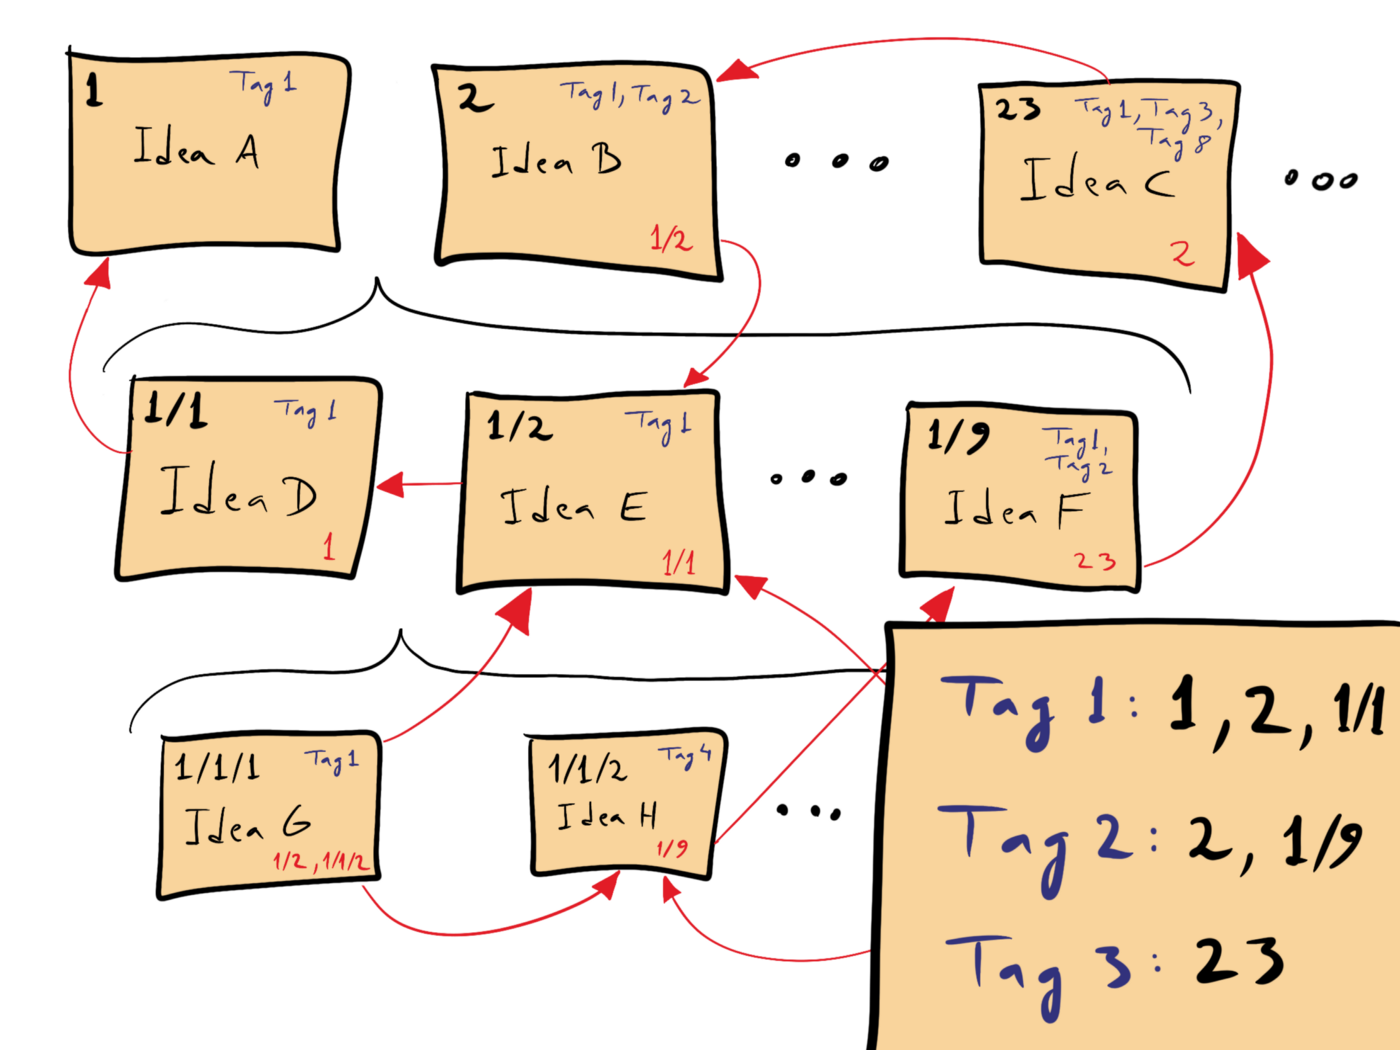
\includegraphics[width=.9\linewidth]{./zk_link.png}
\end{center}

\subsection{Implementation in Emacs}
\label{sec:org893ed86}

\subsubsection{In \texttt{init.el}}
\label{sec:orgab5d17d}
\begin{verbatim}
(org
 +roam2
 +noter)
\end{verbatim}


\subsubsection{In \texttt{package.el}}
\label{sec:org98aea88}

\begin{verbatim}
(unpin! org-roam)
(unpin! org-roam-bibtex)
(package! org-roam-ui)
(package! citar)
(package! helm-bibtex)

\end{verbatim}


\subsubsection{In \texttt{config.el}}
\label{sec:org67ab3c1}
\begin{enumerate}
\item \texttt{org-roam}
\label{sec:org76e31b6}
\begin{verbatim}
(after! org-roam
  (setq org-roam-directory (file-truename "~/documents/2022/2022_01_Taller_Emacs/Day_4/roam" ))
  (setq completion-ignore-case t))
\end{verbatim}

\begin{verbatim}
(setq org-roam-capture-templates
        '(("n" "note" plain "%?"
           :target (file+head "%<%Y%m%dT%H%M%S>-${slug}.org"
                              ":PROPERTIES:
:ID: %<%Y%m%dT%H%M%S>
:Time-stamp: <>
:END:
#+TITLE: ${title}
#+DATE: [%<%Y-%m-%d  %H:%M:%S>]")
           :immediate-finish t
           :unnarrowed t
           :jump-to-captured t)
          ("r" "reference" plain "%?"
           :target (file+head "literature/${citekey}.org"
                              ":PROPERTIES:
:ROAM_REFS: @${citekey}
:ID: %<%Y%m%dT%H%M%S>
:Time-stamp: <>
:END:
#+TITLE: ${citekey}: ${title}
#+DATE: [%<%Y-%m-%d  %H:%M:%S>]
#+FILETAGS: literature

- *Author(s)* :: ${author-or-editor}
- *Title*     :: ${title}
- *Tags*      :: ${keywords}
- *URL*       :: ${url}
- *File*      :: [[file:${file}]]

* ${citekey}: Summary
:PROPERTIES:
:END:

* ${citekey}: LN
:PROPERTIES:
:END:

* Fleeting notes
:PROPERTIES:
:ROAM_EXCLUDE: t
:Custom_ID: ${citekey}
:URL: ${url}
:AUTHOR: ${author-or-editor}
:NOTER_DOCUMENT: ${file}
:NOTER_PAGE:
:END:")
           :immediate-finish t
           :unnarrowed t
           :jump-to-captured t)))
\end{verbatim}


\item \texttt{org-roam-bibtex}
\label{sec:orge856efa}
\begin{verbatim}
(after! citar-org
  (setq citar-bibliography '("~/Dropbox/home/documents/2022/2022_01_Taller_Emacs/Day_4/roam/library.bib"))
  (setq org-cite-global-bibliography citar-bibliography)
  (setq bibtex-completion-bibliography citar-bibliography)
  (setq citar-notes-paths '("~/Dropbox/home/documents/2022/2022_01_Taller_Emacs/Day_4/roam/literature/"))
  (setq org-cite-insert-processor 'citar)
  (setq org-cite-follow-processor 'citar)
  (setq org-cite-activate-processor 'citar)
  (setq citar-open-note-function 'orb-citar-edit-note)
  (setq citar-at-point-function 'embark-act)
  ;; Use consult-completing-read for enhanced interface.
  (advice-add #'completing-read-multiple :override #'consult-completing-read-multiple))

(use-package! org-roam-bibtex
  :after org-roam
  :config
  ;; (require 'org-ref)
  (setq orb-preformat-keywords
        '("citekey" "title" "url" "author-or-editor" "keywords" "file"))

  (setq orb-roam-ref-format 'org-cite)

  (setq orb-process-file-keyword t
        orb-file-field-extensions '(".pdf", ".djvu")
        orb-insert-follow-link t))
\end{verbatim}


\item \texttt{org-roam-ui}
\label{sec:orgd9126b3}
\begin{verbatim}
(use-package! websocket
  :after org-roam)

(use-package! org-roam-ui
  :after org-roam
  :config
  (setq org-roam-ui-sync-theme t
        org-roam-ui-follow t
        org-roam-ui-follow-mode t
        org-roam-ui-update-on-save t
        org-roam-ui-open-on-start t))
\end{verbatim}
\end{enumerate}

\subsection{Workflow}
\label{sec:orga3c2437}

\begin{enumerate}
\item Include sources to Zotero: \url{https://www.wisdom.weizmann.ac.il/\~zvika/course2015/announcements/WainerAmericanStatistician1984.pdf}
\item Export bibtex file.
\item Capture the reference.
\item Highlight the pdf (fleeting notes).
\item Create literature notes.
\item Create permanent notes.
\item Link notes.
\item Visualize
\end{enumerate}

\subsection{Optional}
\label{sec:orge3c4190}

\begin{verbatim}
(after! org-roam
  (map! :leader
        (:prefix-map ("r" . "+org-roam")
         :desc "org-roam"             "l" #'org-roam-buffer-toggle
         ;; :desc "org-roam-find-index"  "j" #'(lambda () (interactive) (org-roam-node-visit (org-roam-node-from-id "zk-index-20200615T000001")))
         :desc "org-roam-node-insert" "i" #'org-roam-node-insert
         :desc "org-roam-node-find"   "f" #'org-roam-node-find
         :desc "org-roam-ref-find"    "r" #'org-roam-ref-find
         :desc "org-roam-ui-mode"     "g" #'org-roam-ui-mode
         :desc "org-roam-capture"     "c" #'org-roam-capture))

  (defun org-roam-image-name (fignumber  description ext)
    (concat (org-roam-id-at-point) "-figure-" (number-to-string fignumber) "-" (clean-filename description) "." ext )))
\end{verbatim}
\end{document}